\chapter{Les émotions dans la parole}
\label{chapitre1}
 	«Tout le monde sait ce qu’est une émotion, jusqu’à ce que vous lui demandiez de la définir. A ce moment-là, il semble que plus personne ne sache.» (Fehr \& Russell, 1984)


 \section{Définition de l'émotion}
L'étude de l'émotion humaine est à la croisée de plusieurs domaines dont notamment la psychologie, la physiologie et la linguistique. Sa définition et sa caractérisation est encore aujourd'hui source d'études. En effet, il n'y a pas de consensus clair et établi sur une définition et une théorie qui priment sur les autres~\cite{Kleinginna1981,Strongman1996}. Néanmoins les scientifiques s'accordent à dire que les émotions sont des facteurs explicatifs des comportements de l'humain~\cite{Gorman2003}. Ce qui explique pourquoi les chercheurs persitent à vouloir révéler leurs secrets.

La définition de l'émotion est exprimée différemment en fonction des domaines d'étude. Pour le grand public, le dictionnaire Le Robert~\footnote{https://dictionnaire.lerobert.com/definition/emotion} définit trois sens du mot émotion :
\begin{itemize}
    \item État affectif intense, caractérisé par des troubles divers (pâleur, accélération du pouls, etc.). Par exemple : Être paralysé par l'émotion ; Tu nous as donné des émotions, tu nous as fait peur (familier).
    \item État affectif, plaisir ou douleur, nettement prononcé.
    \item Sensibilité. Par exemple : Interpréter une œuvre avec émotion.
\end{itemize}
Au sein de cette thèse, nous considérons l'émotion selon la deuxième définition. L'émotion est un état temporaire dans lequel se trouve une personne, elle est causée par un sentiment vif ressenti habituellement en réponse à une stimulation de l'environnement. Ce concept assez général regroupe une multitude d'états qui peuvent aller de la joie à la tristesse en passant par la peur et la colère. De nombreuses théories ont été présentées au fil des siècles pour définir l'émotion.

\subsection{Point historique sur les théories de l'émotion}
\begin{figure}
  \centering
  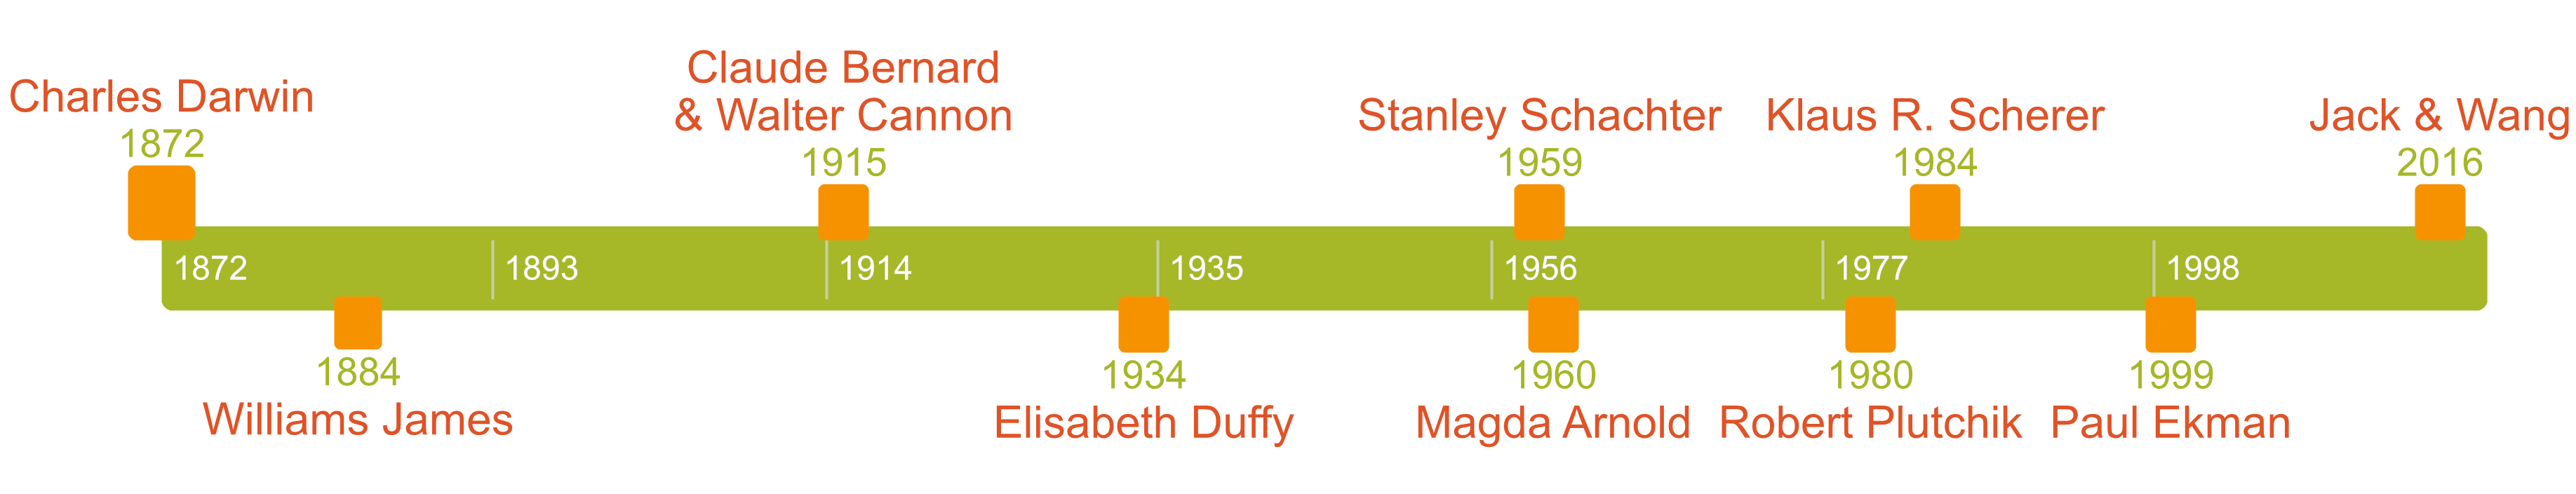
\includegraphics[width=16cm]{./Chapitre1/figures/friseHisto.png}
  \caption{Frise chronologique des grandes théories des émotions selon leur première date de parution}
  \label{fig:Circumplex}
\end{figure}


L'émotion et les états émotionnels, non content de ne pas avoir une unique définition, ont évolué dans leur caractérisation au fil du temps.

Les premières mentions importantes de l'émotion nous viennent d'Aristote qui, au IVe siècle avant J-C, définit l'Être comme une combinaison d'émotion et de raison. Bien plus tard, au XVIe siècle, d'autres philosophes se sont intéressés à l'émotion en la mettant en relation avec la raison. Spinoza théorise que les états émotionnels ont une influence sur le raisonnement humain, tandis que Descartes pense que ces deux notions sont décorrélées.

\subsubsection{Les prémices de Darwin}
L'étude contemporaine des états émotionnels a réellement débuté avec les travaux de Charles Darwin (1872)~\cite{Darwin1872}, qui a défini ses sept principes régissant l'émotion :
\begin{itemize}
    \item les émotions sont innées : elles sont dues à l'Évolution et présentes dès la naissance. Elles se complexifient lorsque la personne grandit.
    \item Elles suivent une continuité phylogénétique : les émotions sont aussi présentes chez les animaux proches de l'être humain, par exemple les primates.
    \item Elles sont dénombrables : on peut caractériser chaque émotion par une des huit catégories définies par Darwin (souffrances, abattement, joie, mauvaise humeur, haine, mépris, surprise et honte) ou par une combinaison de ces dernières.
    \item Elles sont analysables : on peut les caractériser en fonction de l'activité musculaire du visage.
    \item Elles sont reconnaissables : les témoins reconnaissent naturellement l'émotion d'une personne et la traitent en tant qu'information.
    \item Elles sont universelles : comme elles viennent de l'Évolution, elles sont multi-culturelles et leur manifestation est reconnaissable par tous.
    \item Et enfin, elles sont actionnables : \textit{le simple acte de simuler une expression tend à la faire naître dans notre esprit} : nous pouvons ressentir de la joie en nous persuadant que nous sommes heureux.
\end{itemize}

Les émotions servent à la survie de l’espèce et sont définies comme adaptatives. En effet, elles permettent d'adopter une réaction appropriée à un stimulus de l'environnement.

\begin{figure}
  \centering
  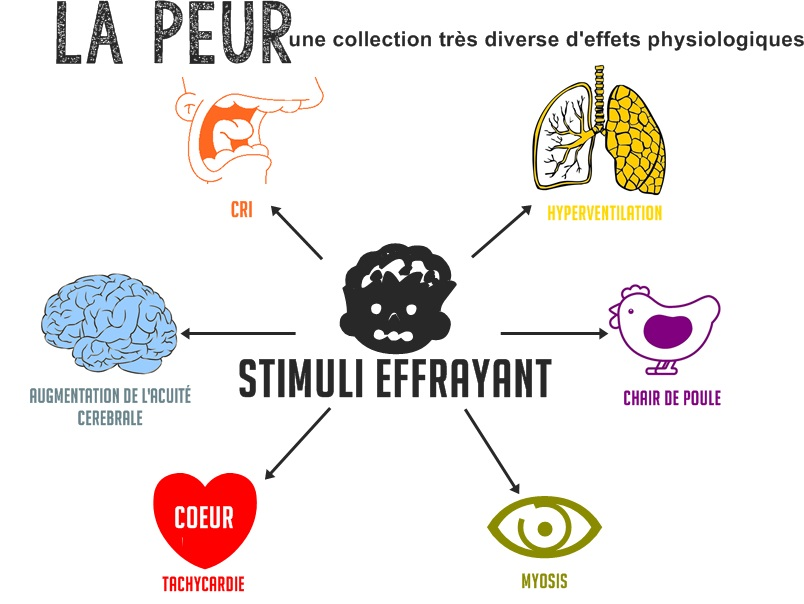
\includegraphics[width=12cm]{./Chapitre1/figures/peur.jpg}
  \caption{Réactions physiologiques du corps devant une situation dangereuse. Image tirée du site www.comprendrelapeur.e-monsite.com.}
  \label{fig:peur}
\end{figure}


Par exemple prenons le cas d'une situation dangereuse : la rencontre avec un animal dangereux, tel un hippopotame. L'homme ressent une émotion en réponse à ce changement d'environnement : la peur. Celle-ci va activer toute une chaîne de réponses biologiques afin d'augmenter les chances de survie. Parmi ces réponses biologiques présentées dans la figure~\ref{fig:peur}, l'augmentation du rythme cardiaque permettant de mieux oxygéner les muscles, et l'agrandissement de l'iris de l'oeil, permettant de mieux voir les mouvements brusques. Ces réponses faciliteront la survie de l'humain qui choisira entre l'attaque et la fuite.

Darwin avance également que certaines émotions, les émotions basiques, sont universelles et innées. Elles sont donc à la fois ressenties et comprises de tous. Cette notion d'émotion fondamentale va longtemps accompagner les théories visant à expliquer l'émotion, mais chaque contributeur définira ses propres émotions primaires.

\subsubsection{L'émotion dite périphérique}
Avec la naissance de la psychologie au XIXe siècle, de nombreuses théories ont émergé pour définir et caractériser l'émotion. Williams James (1884) définit l'émotion comme une conséquence de la réponse physiologique à un stimulus de l'environnement~\cite{James1884}. L'émotion est dite \textit{périphéraliste}, ce qui était considéré auparavant comme la conséquence de l’émotion est ici avancé comme la cause.

Si une personne nous insulte, on ne crie pas parce qu'on est en colère, on est en colère parce qu'on crie. L'émotion se résumerait donc à la prise de conscience des changements qui s'opèrent dans notre corps, que ce soit au niveau de nos muscles, notre respiration, nos viscères... Cela implique que les émotions sont contrôlables, on peut les accentuer ou les inhiber par le simple exercice de sa volonté.

Bien que cette théorie soit en totale rupture avec les conceptions classiques de l'époque, elle va trouver un écho dans le siècle qui suit. Elle sera notamment partiellement validée par les travaux de James Douglas Laird (1974)~\cite{Laird1974} qui traite de l'impact des expressions faciales simulées dans le ressenti des émotions, ou encore par les travaux de Sabine Stepper et Fritz Strack (1993) sur l'impact de la posture~\cite{Stepper1993} ou encore par les travaux de Pierre Philippot (2002)~\cite{Philippot2002} sur l'impact de la respiration.

\subsubsection{L'émotion dite centrale}
En opposition à la théorie de l'émotion périphérique, Claude Bernard et Walter Cannon (1915, 1927) vont définir la notion d’homéostasie~\cite{Cannon1915,Cannon1927}. Étudiant à l'époque le mouvement des viscères, ils ont observé que ces dernières se contractent lorsque le sujet est soumis à de vives émotions, pouvant aller jusqu'à l'arrêt de la digestion lorsque le sujet est soumis à une émotion suffisamment intense. L'émotion est donc un processus qui permet au corps d'interrompre son fonctionnement normal. Cette interruption permet de concentrer les ressources du corps afin d'opérer une réponse adaptée au changement de l'environnement, principalement l'attaque ou la fuite. L'émotion est donc centrale dans le corps, servant de système de mise en alerte de l'organisme.

Ces travaux permettent également de situer la partie du cerveau responsable de l'émotion : les régions sous-corticales~\cite{Cannon1933}. Ces régions sont donc responsables des réponses viscérales, c'est-à-dire des réponses homéostatiques d'urgence mais également du ressenti émotionnel de l'individu en tant qu'expérience subjective.
Les conclusions de ces travaux lanceront l'exploration du cerveau pour trouver les régions responsables des différentes émotions, amenant les neurosciences à s'emparer du domaine de l'émotion~\cite{Bard1934}.

\subsubsection{L'émotion sous forme d'activation}
En parallèle de ces explorations, la notion d'activation va émerger avec Élisabeth Duffy (1934, 1941)~\cite{Duffy1934,Duffy1941}. En effet, maintenant que les émotions sont détectables dans le cerveau humain, elles peuvent être traduites par des mesures du potentiel d'activité. D'un point de vue biologique, les informations sont perçues par le cerveau sous forme de messages nerveux. Ces messages sont en réalité des signaux électriques, encore appelés influx nerveux, qui transitent de neurone en neurone. Ces influx libèrent un potentiel d'activité, que nous savons mesurer.

La théorie des émotions en catégories discrètes comme définie par Darwin est donc réévaluée. En effet, si toutes les émotions peuvent être mesurées en potentiel d'activité de certaines zones du cerveau, la frontière entre les émotions peut être plus perméable que préalablement définie. Cette théorie inscrit donc un tournant dans l'étude des émotions, en introduisant des émotions plus complexes qui ne sont plus définies par un terme, une catégorie ; mais par une mesure de potentiel sur une échelle donnée. Il s'agit là des prémices des théories dimensionnelles aussi appelées théories continues.
Cette théorie sera néanmoins plus difficile à démontrer que prévu, puisque les époux Lacey (1958) ont constaté que toutes les mesures (électro-encéphalogramme, activité des viscères, tension musculaires) ne covarient pas et sont différentes d'un individu à un autre~\cite{Lacey1958}.

\subsubsection{L'émotion en tant que théorie cognitivo-physiologique}
En réponse à ces constatations, Stanley Schachter (1959) a proposé sa théorie cognitivo-physiologique~\cite{Schachter1959,Schachter1962}. Selon lui, nous définissons nos émotions en fonction de la situation dans laquelle nous nous trouvons. En effet, nous devons raisonner pour définir nos propres émotions, en \textit{attribuant} celle-ci à un contexte interne et/ou externe. L'émotion naît donc de deux facteurs : l'activation physiologique et l'attribution cognitive. L'état émotionnel n'est donc plus une simple réponse à un stimulus de l'environnement, elle implique également une part de raisonnement.
\begin{table}[]
\begin{tabular}{|l|l|l|l|l|}
\hline
\multicolumn{1}{|c|}{\textbf{Dimension d’évaluation}} & \multicolumn{1}{c|}{\multirow{2}{*}{\textbf{Colère/Rage}}} & \multicolumn{1}{c|}{\multirow{2}{*}{\textbf{Peur}}} & \multicolumn{1}{c|}{\multirow{2}{*}{\textbf{Tristesse}}} & \multicolumn{1}{c|}{\multirow{2}{*}{\textbf{Joie}}} \\
\multicolumn{1}{|c|}{\textbf{émotionnelle}}           & \multicolumn{1}{c|}{}                                      & \multicolumn{1}{c|}{}                               & \multicolumn{1}{c|}{}                                    & \multicolumn{1}{c|}{}                               \\ \hline
\multicolumn{5}{|c|}{\textbf{Nouveauté}}                                                                                                                                                                                                                                                  \\ \hline
Soudaineté                                            & haut                                                       & haut                                                & bas                                                      & bas                                                 \\ \hline
Familiarité                                           & bas                                                        & bas                                                 & bas                                                      & ouvert                                              \\ \hline
Prévisibilité                                         & bas                                                        & bas                                                 & ouvert                                                   & moyen                                               \\ \hline
\multicolumn{5}{|c|}{\textbf{Valence}}                                                                                                                                                                                                                                                    \\ \hline
intrinsèque                                           & ouvert                                                     & bas                                                 & ouvert                                                   & haut                                                \\ \hline
\multicolumn{5}{|c|}{\textbf{Rapport aux buts/besoins}}                                                                                                                                                                                                                                   \\ \hline
Pertinence                                            & haut                                                       & haut                                                & haut                                                     & moyen                                               \\ \hline
Degré de certitude dans la                            & \multirow{2}{*}{très haut}                                 & \multirow{2}{*}{haut}                               & \multirow{2}{*}{très haut}                               & \multirow{2}{*}{très haut}                          \\
prédiction des conséquences                           &                                                            &                                                     &                                                          &                                                     \\ \hline
Congruence avec les attentes                          & dissonant                                                  & dissonant                                           & ouvert                                                   & consonnant                                          \\ \hline
Opportunité                                           & obstruction                                                & obstruction                                         & obstruction                                              & facilitation                                        \\ \hline
Urgence                                               & haut                                                       & très haut                                           & bas                                                      & très bas                                            \\ \hline
\multicolumn{5}{|c|}{\textbf{Potentiel de maîtrise}}                                                                                                                                                                                                                                      \\ \hline
Causalité : agent                                     & autrui                                                     & autrui/naturel                                      & ouvert                                                   & ouvert                                              \\ \hline
Causalité : motivation                                & intentionnel                                               & ouvert                                              & hasard                                                   & intentionne                                         \\ \hline
Contrôle                                              & haut                                                       & ouvert                                              & très bas                                                 & ouvert                                              \\ \hline
Puissance                                             & haut                                                       & très bas                                            & très bas                                                 & ouvert                                              \\ \hline
Ajustement                                            & haut                                                       & bas                                                 & moyen                                                    & haut                                                \\ \hline
\multicolumn{5}{|c|}{\textbf{Accord avec les normes}}                                                                                                                                                                                                                                     \\ \hline
Standards externes                                    & ouvert                                                     & ouvert                                              & ouvert                                                   & ouvert                                              \\ \hline
Standards internes                                    & bas                                                        & ouvert                                              & ouvert                                                   & ouvert                                              \\ \hline
\end{tabular}
\label{tab:Scherer}
\caption{Grille d'évaluation des premiers travaux de Scherer pour définir une émotion en fonction des 5 questionnements. In P. Philippot. (2007). Emotion et psychothérapie (pp.11-64). La catégorie ouvert est utilisé lorsque l'évaluation peut etre de différente catégorie. Par exemple, pour la joie, l'élément déclencheur peut être quelque chose de connu ou non (Familiarité). En rapport aux buts/besoins, les opportunités peuvent être obstruées (émotions négatives) ou facilitées (émotions positives).}
\end{table}


\subsubsection{L'émotion avec la théorie de l'évaluation}
En s'appuyant sur ces travaux, Magda Arnold (1960) va amorcer la théorie de l'évaluation cognitive (appraisal en anglais)~\cite{Arnold1960}, qui va prendre de l'ampleur avec les travaux de Scherer (1984)~\cite{Scherer1984}. Ce dernier considère que l'évaluation d'une situation est définie par cinq questionnements :
\begin{itemize}
  \item Est-ce que la situation est nouvelle ? (nouvelle/ancienne)
  \item Est-ce qu'elle suscite du plaisir intrinsèque ? (agréable/désagréable)
  \item Est-ce qu'elle est pertinente ? (aidante/gênante)
  \item Est-ce qu'on sait y faire face ? (on a le contrôle/ on n'a pas le contrôle)
  \item Est-ce que c'est compatible avec les normes ? (compatible avec les normes sociales et ses propres convictions)
\end{itemize}

C'est en réponse à ces cinq questions que Scherer va proposer cinq dimensions pour représenter l'émotion : la nouveauté, la valence, le rapport aux buts, le potentiel de maîtrise et l'accord avec les normes. La grille d'évaluation, présentée dans le tableau 1.1
%~\ref{tab:Scherer}
, permet de caractériser l'état émotionnel d'un individu en quatre émotions : la colère/rage, la peur, la tristesse et la joie.
On voit sur ce tableau la description de la joie par exemple. Pour Philippot~\cite{Philippot2002}, elle se caractérise par une situation peu soudaine et assez prévisible, qui suscite un fort plaisir intrinsèque, qui est une situation plutôt aidante (donc elle a une forte relation avec les attentes du sujet), sur laquelle on a plus ou moins de contrôle et qui est plus ou moins compatible avec les normes.

Toutes ces théories sont encore aujourd'hui étudiées et affinées en fonction des situations d'étude des émotions. Mais aucune n'est reconnue comme étant une vérité absolue. C'est en se basant sur toutes ces théories et ces travaux que le domaine de l'informatique va alors se mettre au service de l'étude de l'émotion.


\section{Représentation courante des émotions à but d'automatisation de traitement}
Comme nous l'avons vu précédemment, il n'y a pas de consensus sur une définition ou même une caractérisation des états émotionnels~\cite{Kleinginna1981}. Cela peut être expliqué par notamment, la multitude de domaines qui sont intéressés par l'émotion (psychologie, physiologie, linguistique, phonologie, sciences cognitives, informatique...) ou encore par la part non négligeable de la subjectivité du domaine et donc de la grande variabilité inter-sujet.

Néanmoins dans le domaine de l'informatique, nous faisons principalement la distinction entre deux grands courants : l'émotion définie par des états discrets et/ou par des états continus. En effet, afin d'automatiser le traitement des émotions, il est nécessaire de se tenir à une théorie algorithmiquement descriptive. Il faut donc définir des représentations émotionnelles en adéquation avec les besoins exprimés pour une tâche donnée. Ce domaine d'étude est appelé informatique affective ou affective computing en anglais. Décrit dans les travaux de Rosalind Picard en 1995~\cite{Picard2000}, ce domaine reste très récent et en plein développement.

Au sein de cette thèse, notre tâche est la détection et la caractérisation automatique d'émotions contenues dans la parole. Nous proposons donc de rappeler la définition de ces deux ensembles de théorie qui sont \textit{dans une guerre centenaire} l'une contre l'autre~\cite{Lindquist2013}, donnant naissance à la multitude de définitions que nous lui connaissons.

\subsection{Théorie des émotions discrètes}
Comme a dit Izard : \textit{... people need the category label of joy (or its equivalent) to explain the pride of achievement, sadness to explain the experience of a life-changing loss, anger to explain the frustration of blocked goal responses, and fear to explain flight to one another for safety}
%\textit{people need the category label of fear to explain flight to one another for safety, anger to explain the frustration of blocked goal responses, joy (or its equivalent) to explain the pride of achievement, and sadness to explain the experience of a life-changing loss}
~\cite{Izard2007}. Nous avons donc besoin de pouvoir regrouper des états émotionnels pour définir des catégories, ce qui nous aide à mieux expliciter nos émotions.

La théorie des émotions discrètes considère qu'il existe un nombre défini d'émotions qui peuvent être formellement caractérisées. Certaines d'entre elles sont définies comme étant \textit{basiques, primaires} ou \textit{basales} et permettent, en se combinant, d'exprimer des émotions plus \textit{complexes}. Elles sont caractérisées par un ressenti, des expressions comportementales et physiologiques qui sont spécifiques à chaque individu mais reconnaissables par tous. Ces trois aspects permettent de caractériser chaque émotion. Certaines émotions sont admises par tous (colère, dégoût, joie, peur, surprise, tristesse), d'autres sont plus discutées~\cite{Cosnier1994}.

Historiquement Charles Darwin est l'un des premiers à définir ces émotions basiques, au nombre de cinq (la colère, le dégoût, la joie, la peur et la tristesse), dans sa théorie de l'évolution.
Même s'il y a des théories qui ont plus d'adeptes que d'autres, il n'y a pas de théorie qui fait consensus au sein de la communauté qui permettrait de définir ces émotions basiques, de les dénombrer ou d'expliquer leur combinaison en émotions complexes. D'autant plus que les émotions et leurs manifestations n'ont eu de cesse d'évoluer en même temps que nos sociétés.

\begin{table}[]
\begin{tabular}{|l|l|}
\hline
\textbf{Auteyrs} & \textbf{Émotions basiques} \\ \hline
Darwin (1872)       & colère, peur, joie, tristesse, dégoût                                                               \\ \hline
James (1884)        & peur, douleur/chagrin, amour, rage                                                                  \\ \hline
Arnold (1960)       & \begin{tabular}[c]{@{}l@{}} colère, aversion, haine, peur, découragement, \\
                              courage, amour, désir, espoir, désespoir, tristesse\end{tabular}                            \\ \hline
Tomkins (1962)      & rage, peur, joie, angoisse, dégoût, surprise , intérêt, honte                                      \\ \hline
Izard (1971)        & \begin{tabular}[c]{@{}l@{}} intérêt, joie, surprise, tristesse, colère, dégoût, mépris, \\
                              auto-hostilité, peur, honte, timidité, culpabilité \end{tabular}                            \\ \hline
Plutchik (1980)     & \begin{tabular}[c]{@{}l@{}} colère, peur, joie, tristesse, dégoût, surprise,  \\
                              acceptation, anticipation \end{tabular}                                                     \\ \hline
Frijda (1986)       & désir, intérêt, bonheur, surprise                                                                   \\ \hline
Oatley \& Jonhson-Laird (1987)    & colère, dégoût, inquiétude, bonheur, tristesse                                        \\ \hline
Gray (1990)         & rage, terreur, anxiété, joie                                                                        \\ \hline
Ekman (1999)        & colère, peur, joie, tristesse, dégoût, surprise                                                     \\ \hline
\begin{tabular}[c]{@{}l@{}}Jack (2016), Gu (2015)
  \\ et Wang (2016)\end{tabular}   & peur, colère, joie, tristesse                                                        \\ \hline
\end{tabular}
\label{tab:EmotionsBasiques}
\caption{Définition des émotions basiques selon différents auteurs}
\end{table}


De nombreux auteurs ont proposés des émotions primaires : Paul Ekman propose les populaires six émotions faciales basiques (colère, dégoût, joie, peur, surprise, tristesse) qu'on appellera par la suite les \textit{Big Six}~\cite{Ekman1999}, tandis que Robert Plutchik en propose huit (anticipation, colère, confiance, dégoût, joie, peur, surprise, tristesse)~\cite{Plutchik1980}. On peut constater que la définition de ces émotions basiques est encore aujourd'hui source de discussions : Rachael Jack, Simeng Gu et Fushun Wang~\cite{Jack2016,Gu2015,Wang2016} ont proposé quatre émotions basiques (la colère, la joie, la peur et la tristesse) en 2015 et 2016. Le tableau 1.2
%~\ref{tab:EmotionsBasiques}
 liste les catégories des émotions primaires selon leurs auteurs. On peut remarquer néanmoins que l'on considère de quatre à douze émotions basiques, et que sur ces onze auteurs, on a une moyenne de six à sept émotions basiques. On retrouve également les émotions colère, joie, peur et tristesse dans presque toutes les théories.

Paul Ekman a joué un grand rôle dans la diffusion de cette théorie grâce, entre autre, à la création de la méthode \textit{Facial Action Coding System} (FACS)~\cite{Ekman1978}. Utilisée dans des domaines grand public tel que la télévision avec la série Lie to Me, cette méthode permet de définir l'émotion à partir de l'expression faciale d'un individu. Il a notamment décrit les neuf caractéristiques d'une émotion basique~\cite{Ekman1999}, inspirée de toutes les autres théories, qui seront globalement repris par tous les autres auteurs :
\begin{itemize}
  \item Les signaux émotionnels sont universels : les émotions de base sont reconnues par tout le monde, quelque soit sa culture ou son origine.
  \item Il existe des expressions communes aux hommes et aux autres primates : nous sommes capables d'identifier la colère chez les Bonobos par exemple.
  \item Chaque émotion est caractérisée par un ensemble de comportements physiologiques comme exprimé par la figure~\ref{fig:Ekman1983}. Par exemple, un individu ayant un rythme cardiaque élevé et une température cutanée élevée ressent de la colère.
  \begin{figure}
  \centering
  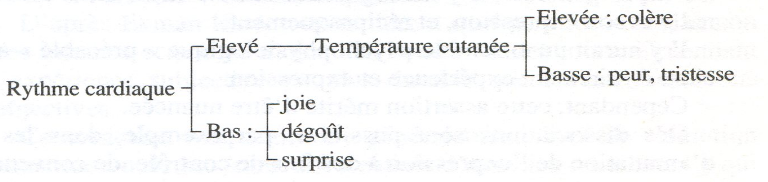
\includegraphics[width=10cm]{./Chapitre1/figures/Ekman1983.png}
  \caption{Traduction de la figure extraite de l'article de Paul Ekman et al.~\cite{Ekman1983} décrivant un arbre de décision pour déterminer l'émotion retrouvée sur le visage.}
  \label{fig:Ekman1983}
\end{figure}

  \item Il existe des éléments déclencheurs d'émotion qui sont universels : controversée, cette caractéristique stipule que des types de situations donnés provoqueront la même émotion donnée chez tout sujet.
  \item Les réactions émotionnelles sont cohérentes : il y a un lien établi et connu entre une expérience émotionnelle et son expression physiologique et réciproquement.
  \item L'émotion engendre une réaction rapide : une fraction de seconde pour les réactions physiologiques et quelques millisecondes pour les mimiques~\cite{Ekman1978}.
  \item L'émotion est limitée dans le temps : la durée d'une émotion n'excède pas la minute.
  \item L'émotion n'est pas contrôlée : elle frappe soudainement, n'étant ni volontaire ni raisonnée. Un individu peut essayer de contrôler les manifestations de l'émotion : il a été observé que la posture et les mimiques sont plus contrôlables que la voix. Les réactions viscérales sont quant à elles très peu contrôlables.
  \item L'émotion est spontanée : elle n'est pas choisie et ne peut pas vraiment être évitée. Toutefois son anticipation peut réduire son intensité. Par exemple devant un film d'horreur, le sujet s'attend à avoir peur, ce qui permet de réduire l'intensité de cette peur.
\end{itemize}

\begin{figure}
  \centering
  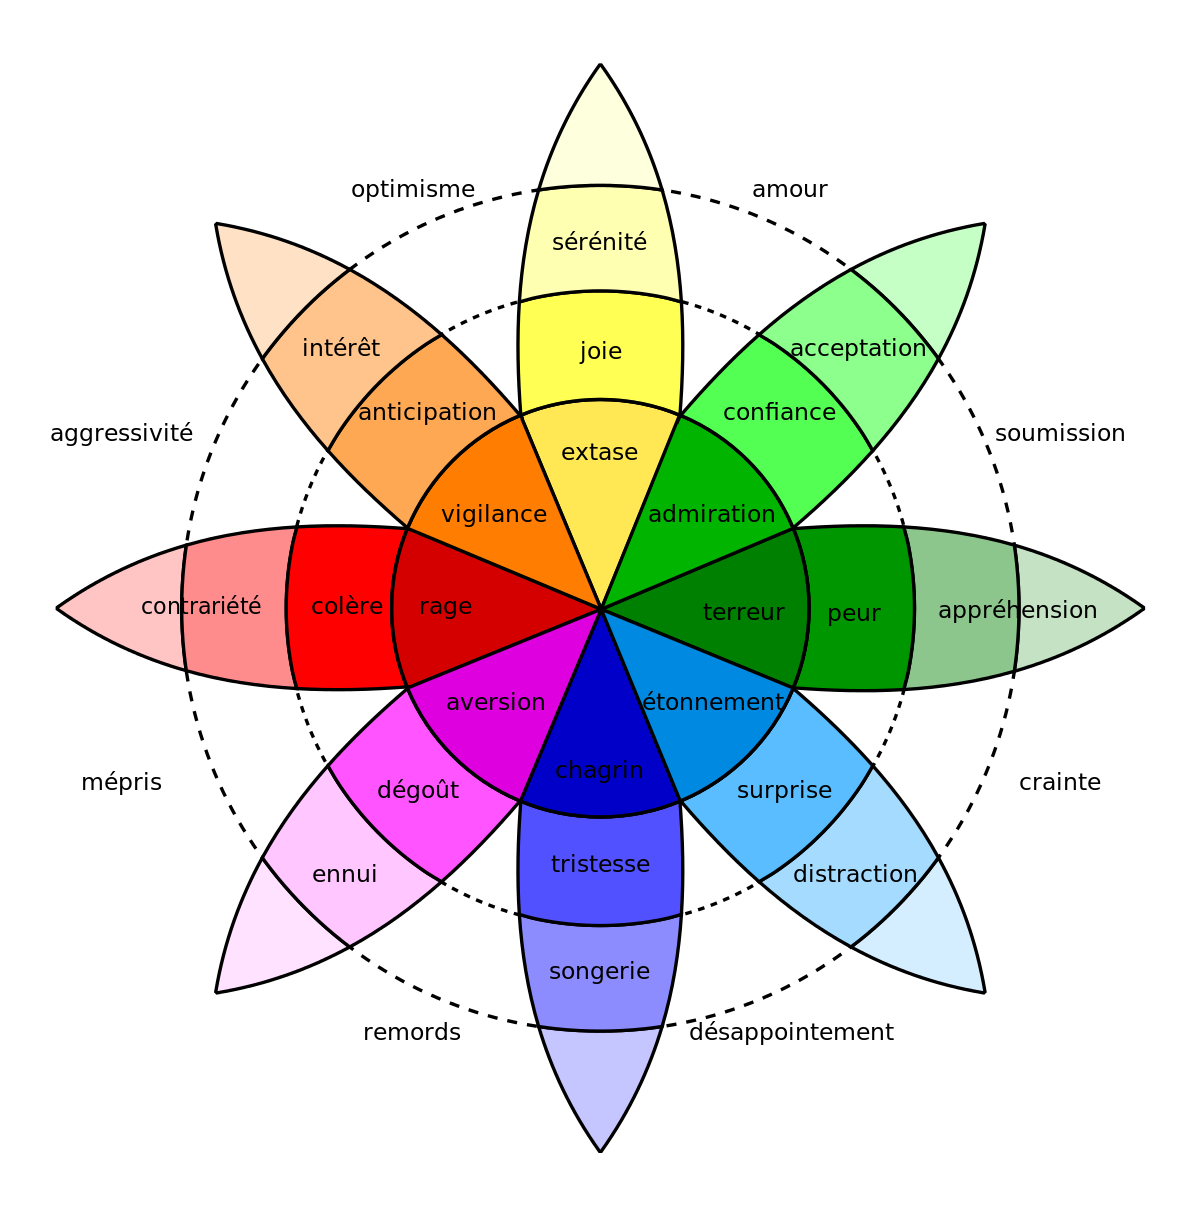
\includegraphics[width=12cm]{./Chapitre1/figures/Plutchik.png}
  \caption{Roue de Plutchik qui définit les émotions complexes à partir d'émotions basiques.}
  \label{fig:Plutchik}
\end{figure}


Ces émotions primaires peuvent également se combiner pour donner des émotions dites \textit{complexes}, qui permettent de nuancer les états émotionnels. C'est notamment le cas avec la roue de Plutchik, présentée dans la figure~\ref{fig:Plutchik}, qui dénombre 32 émotions issues en huit émotions primaires selon leur intensité~\cite{Plutchik1980}. Par exemple une joie très intense correspond à un sentiment d'extase, alors qu'une colère de faible intensité correspond à de la contrariété.

De plus, on parle également d'émotions secondaires afin de décrire des émotions qui ne sont pas innées, mais qui sont apprises pendant le développement de la personne. Paul Ekman définit ainsi neuf émotions secondaires, plus complexes et plus difficiles à identifier (la culpabilité, l'embarras, le mépris, la complaisance, l'enthousiasme, la fierté, le plaisir, la satisfaction et la honte). Elles marquent des différences d'expression en fonction des cultures et des individus. Louis Charland (1995)~\cite{Charland1995} et Antonio Damasio (1999)~\cite{Damasio1999} ont notamment contribué à analyser les différences culturelles de ces émotions secondaires.

Pour résumer, ces théories discrètes caractérisent des émotions par des catégories telles que la joie et la peur. Elles sont observables par tous et limitées dans le temps. Elles peuvent se combiner pour définir des émotions plus complexes.
D'autres théories ont émergé au fil des années, pour définir les émotions. En effet, certains ont trouvé que les émotions en catégories discrètes étaient trop limitantes pour tout représenter. %Ces auteurs ont donc proposé que l'émotion peut être définie par de nombreuses théories continues.


\subsection{Théorie des émotions continues}
Dans la vie courante, il est bien plus facile et coutumier de se référer à des catégories d'émotion telles que la joie ou la tristesse pour décrire ce que l'on ressent. Par exemple, lorsque l'on veut communiquer son état émotionnel à un interlocuteur, on aura tendance à le nommer. Toutefois, une autre façon de définir les émotions est de les inscrire dans des espaces continus, permettant de s'affranchir des contraintes des catégories définies. Il est difficile de déterminer des frontières entre les différentes émotions : les frontières sont ressenties différemment par tout le monde~\cite{Busso2012}. Le manque de frontière dure peut expliquer l'émergence des recherches sur des théories continues pour définir l'émotion. Si l'on s'en réfère aux travaux de Lisa Feldman-Barrett (2006)~\cite{Feldman2006}, les catégories «représente(nt) maintenant un obstacle majeur à la compréhension de ce que sont les émotions et de comment (les émotions) fonctionnent». En effet, les catégories limitent les possibilités pour exprimer des émotions.

\begin{figure}
  \centering
  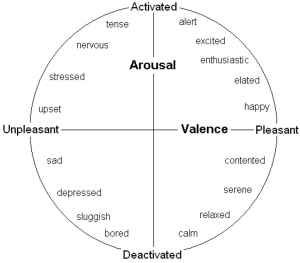
\includegraphics[width=8cm]{./Chapitre1/figures/Circumplex.png}
  \caption{Le modèle circumplex de Russell}
  \label{fig:Circumplex}
\end{figure}


La théorie des émotions continues, aussi appelées dimensionnelles, a été introduite par les travaux de Wilhelm Wundt (1902)~\cite{Wundt1902} et Harold Schlosberg (1954)~\cite{Schlosberg1954}. Les émotions peuvent être décrites selon trois dimensions indépendantes nommées en fonction de leur extremum : agréable-désagréable, tendu-détendu et agité-calme. Grâce à ces trois dimensions, chaque émotion ressentie par un individu peut être décrite comme une combinaison pondérée de ces trois axes. Cependant certaines émotions peuvent se placer au croisement des axes de différentes manières. La joie est agréable, plutôt détendue mais peut être agitée ou calme. Comme ces dimensions se chevauchent, ces dernières ont laissé place au modèle du Circumplex, présenté dans la figure~\ref{fig:Circumplex}, de James Russell en 1980~\cite{Russell1980}, devenant la théorie principale permettant de décrire les émotions de façon continue. Ce modèle permet de placer toutes les émotions au sein d'un cercle dont l'abscisse définie la valence de l'émotion (positive-négative) et l'ordonnée définie l'activation (faible-fort). En effet, on peut donc donner une polarité et une intensité à chaque émotion : la tristesse est définie par une valence négative et une faible activation.

Afin de mieux discriminer des émotions qui ont des mêmes valences et des activations comme par exemple la peur et la colère, d'autres axes ont également été ajoutés sur ce modèle par René Scherer (2005) comme la dominance (dominance-soumission) et l'imprévisibilité (faible-forte)~\cite{Scherer2005}, comme illustré dans la figure~\ref{fig:Genova}. Par exemple, on peut voir que la mélancolie (melancholic) a une valence neutre et une faible activation, tandis que la déception (disappointed) a une valence très négative et une activation neutre.
\begin{figure}
  \centering
  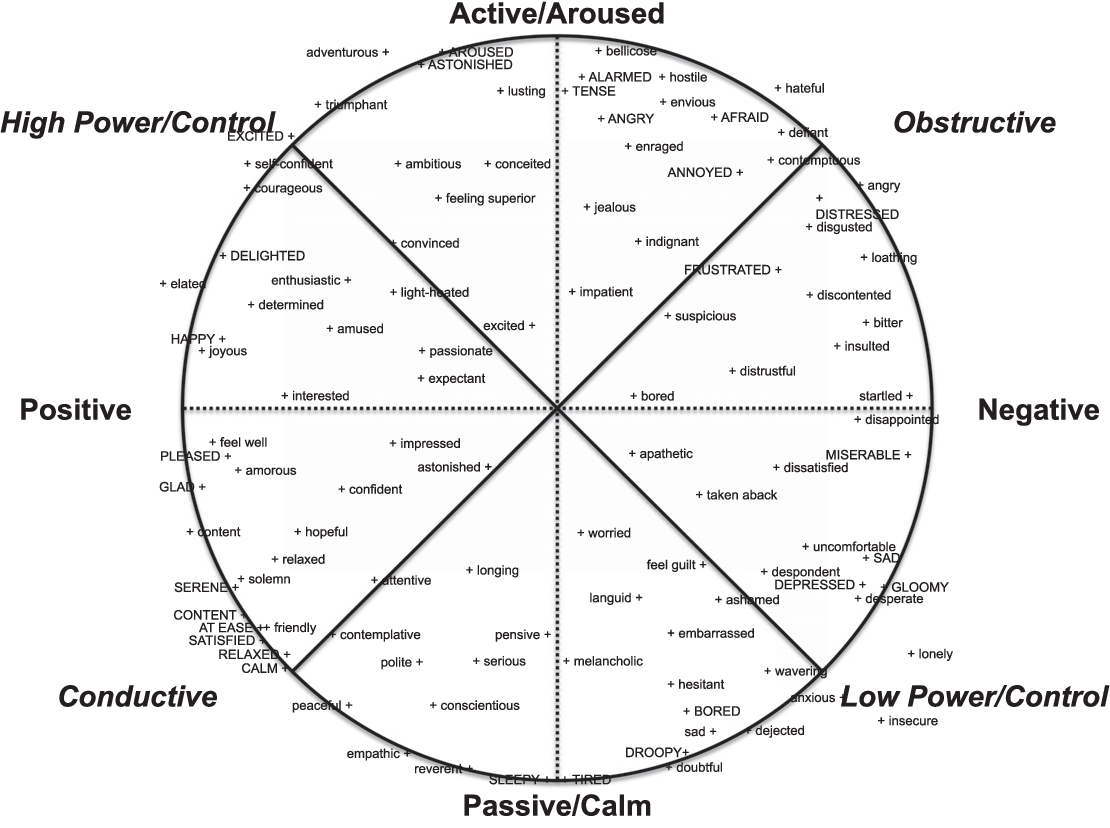
\includegraphics[width=18cm]{./Chapitre1/figures/Genova.png}
  \caption{La roue des émotions de Genève définie par Scherer, qui nomme des émotions (primaires ou secondaires) dans des dimensions continues.}
  \label{fig:Genova}
\end{figure}


D'autres systèmes dimensionnels existent, allant de deux à cinq dimensions, qui ont été crées en fonction des besoins applicatifs~\cite{Mehrabian1980,Cochrane2009}. Toutes ces dimensions peuvent être discrétisées par des systèmes de graduation, permettant notamment de faire le lien avec les théories discrètes.

En ce qui concerne les études menées sur les émotions continues dans le domaine de l'informatique, il y a une forte prévalence des dimensions de valence et d'activation quel que soit le support utilisé (la voix, le texte, la vidéo ou des données physiologiques). En effet, elles sont facilement identifiables par l'humain et reposent sur des caractéristiques automatiquement reconnaissables.
Toutes ces différentes théories permettant de décrire les états émotionnels se rejoignent sur un fait : les émotions sont perceptibles chez les individus de différentes manières.
%Au sein de cette thèse, nous avons décidé de nous appuyer sur la théorie des émotions continues, afin de répondre à la problématique industrielle qui est sensible à l'évolution temporelle de l'intensité de la satisfaction et la frustration.

\section{L'émotion dans la parole}
%Si nous nous replaçons dans le contexte de cette thèse, notre objectif est de décrire l'émotion humaine lors de conversations tenues entre un client et un agent dans un cadre défini par un appel téléphonique en centre d'appels. Nous n'avons donc que la voix comme axe d'analyse pour en retirer les états émotionnels des intervenants.
Un des supports universels vecteur de l'émotion est la voix humaine, et par extension la parole.
La voix est produite par l'appareil phonatoire de l'émetteur et elle est reçue par l'appareil auditif du recepteur. Ce processus est considérée comme un canal de communication selon la théorie de Claude Shannon (1948) ~\cite{Shannon1948}. Ce canal permet de faire passer un message entre un émetteur (ici le locuteur) et un récepteur (ici l'écoutant).

Les appareils phonatoires et auditifs sont la base de la communication orale entre deux individus. L'appareil phonatoire décrit l'ensemble des phénomènes anatomiques qui sont impliquées dans la production des vibrations acoustiques donnant naissance à la parole. Ces phénonèmes sont, par exemple, la création d'un son par la vibration des cordes vocales et le contrôle du souffle ou encore la modulation de ce son par la bouche et par le nez.

La parole peut etre découpée en sous-unités phoniques que l'on appelle des phonèmes. Ces derniers, à ne pas confondre avec des syllabes, permettent de composer l'ensemble des sonorités nécessaires à l'énonciation de parole.
%Par exemple, le mot 'émotion' utilise six phonèmes : /e/ (é), /m/ (m), /ɔ/ (o), /s/ (s), /i/ (i) et /ɔ̃/ (on).
Par exemple, le mot \textit{émotion} utilise six phonèmes : /é/, /m/, /o/, /s/, /i/ et /on/.
Il est important de noter que chaque langue possède sa propre palette de phonèmes. Le français par exemple utilise 36 phonèmes, tandis que l'anglais en utilise 44.

L'appareil auditif, situé dans la boîte cranienne, est composé de tout ce qui permet à l'individu d'entendre et d'écouter la parole. Pour ce qui est de l'oreille, elle est constituée de trois parties :
\begin{itemize}
  \item l'oreille externe : un conduit qui permet de transmettre les vibrations acoustiques,
  \item l'oreille moyenne : qui permet de transformer le signal pour qu'il puisse être conduit dans un environnement liquide en utilisant les osselets,
  \item et l'oreille interne : qui transforme les vibrations en influx nerveux grâce à la cochlée.
\end{itemize}
C'est cet appareil qui permet à un interlocuteur de recevoir un message.

Les informations communiquées par ce canal peuvent être notamment divisées en deux catégories : le linguistique et le para-linguistique.
Le linguistique va décrire le langage en tant que succession de mots tandis que le para-linguistique va définir tout ce qui n'est pas du message verbal. Par exemple, dans la vie de tous les jours, \textit{Bonjour, je voudrais une baguette de pain} correspond au message linguistique, tandis que l'hésitation vocale ou le raclement de gorge font partie du domaine para-linguistique.

Shirley Weitz (1974)~\cite{Weitz1974} explique que le para-linguistique s'intéresse \textit{à la façon dont quelque chose est dit, pas à ce qui est dit}. Globalement, on considère du domaine du para-linguistique dans la parole, l'accent, la hauteur de la voix, le volume, la vitesse de parole, la modulation, la prosodie et la fluidité de l'élocution.
La définition du paralangage étant évolutive, il est naturel que sa définition reste imprécise comme l'indique Peter Matthews dans son dictionnaire de la linguistique~\cite{Matthews2014}.

La prosodie est définie par l'ensemble des phénomènes accoustiques qui accompagnent le discours, tout en n'étant pas du discours. C'est un élément de la partie para-linguistique de la parole. La prosodie est généralement définie par trois paramètres très importants~\cite{Srinivasan2003,Dohen2004}, bien qu'ils ne fassent pas consensus :
\begin{itemize}
  \item L'intonation de la parole. Elle peut être analysée par le contour de la fréquence fondamentale (F0) de la parole, qui correspond à l'inverse de la période d'un son périodique. On utilise également l'évolution temporelle de la F0 pour définir l'intonation.
  \item Le rythme de la parole est lié au temps nécessaire à l'émission d'un segment de parole, et donc à la durée. On peut également parler de débit.
  \item L'intensité de la parole est définie par l'énergie  par unité de temps contenue dans le signal.
\end{itemize}
L'étude para-linguistique d'un discours par le biais de la prosodie nous permet de percevoir notamment l'état émotionel d'un locuteur de façon naturelle. Comme il s'agit du sujet principal de cette thèse, le chapitre 3 revient plus en détail sur la relation entre la voix et les émotions. Mais la voix n'est pas la seule modalité véhiculant des indices émotionnels. Grâce à des outils de plus en plus performants, la parole peut être transformée en texte.

\section{L'émotion dans le texte}
Avec le développement des nouvelles technologies et le nombre de communications écrites toujours grandissant, il devient de plus en plus utile de mieux cerner les informations contenues dans ces messages. En plus de l'aspect sémantique, c'est-à-dire de la compréhension du sujet et du discours tenu dans les messages textuels, il est également possible d'exprimer des états émotionnels~\cite{Hancock2007,SchwarzFriesel2015}. Par exemple, sur les réseaux sociaux, il n'est pas rare de retrouver des messages aux opinions très tranchées sur des sujets, dans lesquels l'individu va montrer son engagement, sa colère ou son soulagement.

Le texte écrit vient avec ces propres codes, en fonction du média utilisé, pour exprimer les états émotionnels. Traditionnellement, l'émotion va se retrouver dans la morphologie du discours, le lexique employé, la syntaxe utilisée et l'aspect figuratif ou non de l'énoncé (par exemple le sarcasme)~\cite{Sailunaz2018}.

En plus de la construction sémantique des mots et des phrases, la ponctuation ou les émoticônes peuvent apporter leur concours pour exprimer des émotions. Par exemple, la répétition de plusieurs points d'interrogation peut traduire la stupéfaction ou l'incompréhension~\cite{Thurlow2013}. L’émoticône :) ( deux points, parenthèse fermante) va permettre d'exprimer la joie ou l'approbation selon le contexte~\cite{Provine2007}.

La détection d'émotion dans le texte peut être réalisée principalement selon les méthodes suivantes :
\begin{itemize}
  \item L'approche basée sur les mots clés~\cite{Ma2005,Liu2003}. Pour détecter la joie, on recherche tous les mots qui sont du champ lexical de la joie (joie, heureux, content...) dans le texte. Cette approche est basée sur l'hypothèse que tous les mots sont indépendants. Le principal inconvénient vient de cette hypothèse. En effet, entre les phrases \textit{je suis heureux} et \textit{je ne suis pas heureux}, cette approche détecte de la joie dans les deux cas, ce qui est faux.
  \item L'approche basée sur des règles~\cite{AlMasum2007,Chaumartin2007}. Pour détecter la joie, on va mettre en place une série de règles en utilisant ou non le champ lexical de la joie et une série de règles. Par exemple, pas de négation dans le segment ou de mot appartenant au champ lexical de la tristesse. Cette approche peut vite devenir complexe, car il faut de nombreuses règles qui ne se contredisent pas pour arriver à une reconnaissance performante.
  \item L'approche basée sur l'apprentissage. Cette approche sera développée dans le chapitre 3.
\end{itemize}

De nombreuses applications peuvent découler de l'analyse des émotions en partant du texte. En effet, le nombre d’interactions entre un humain et une machine ne cesse d'augmenter tous les jours. Permettre aux machines de mieux comprendre et identifier les besoins de l'humain reste donc une préoccupation majeure de notre époque. Les émotions ont donc un rôle à jouer dans cette communication~\cite{Picard2000}. Outre la parole et le texte, il existe d'autres comportements reconnaissables qui accompagnent l'émotion.

\section{Les autres marqueurs de l'émotion chez l'humain}
Outre la présence de marqueurs émotionnels dans la voix, d'autres indicateurs peuvent être relevés dans les expressions faciales et dans les réponses physiologiques. Il est donc possible d'étudier l'état émotionnel d'une personne à partir d'une vidéo ou de relevés physiologiques.

\subsection{Les marqueurs faciaux et comportementaux de l'émotion}

\begin{figure}
  \centering
  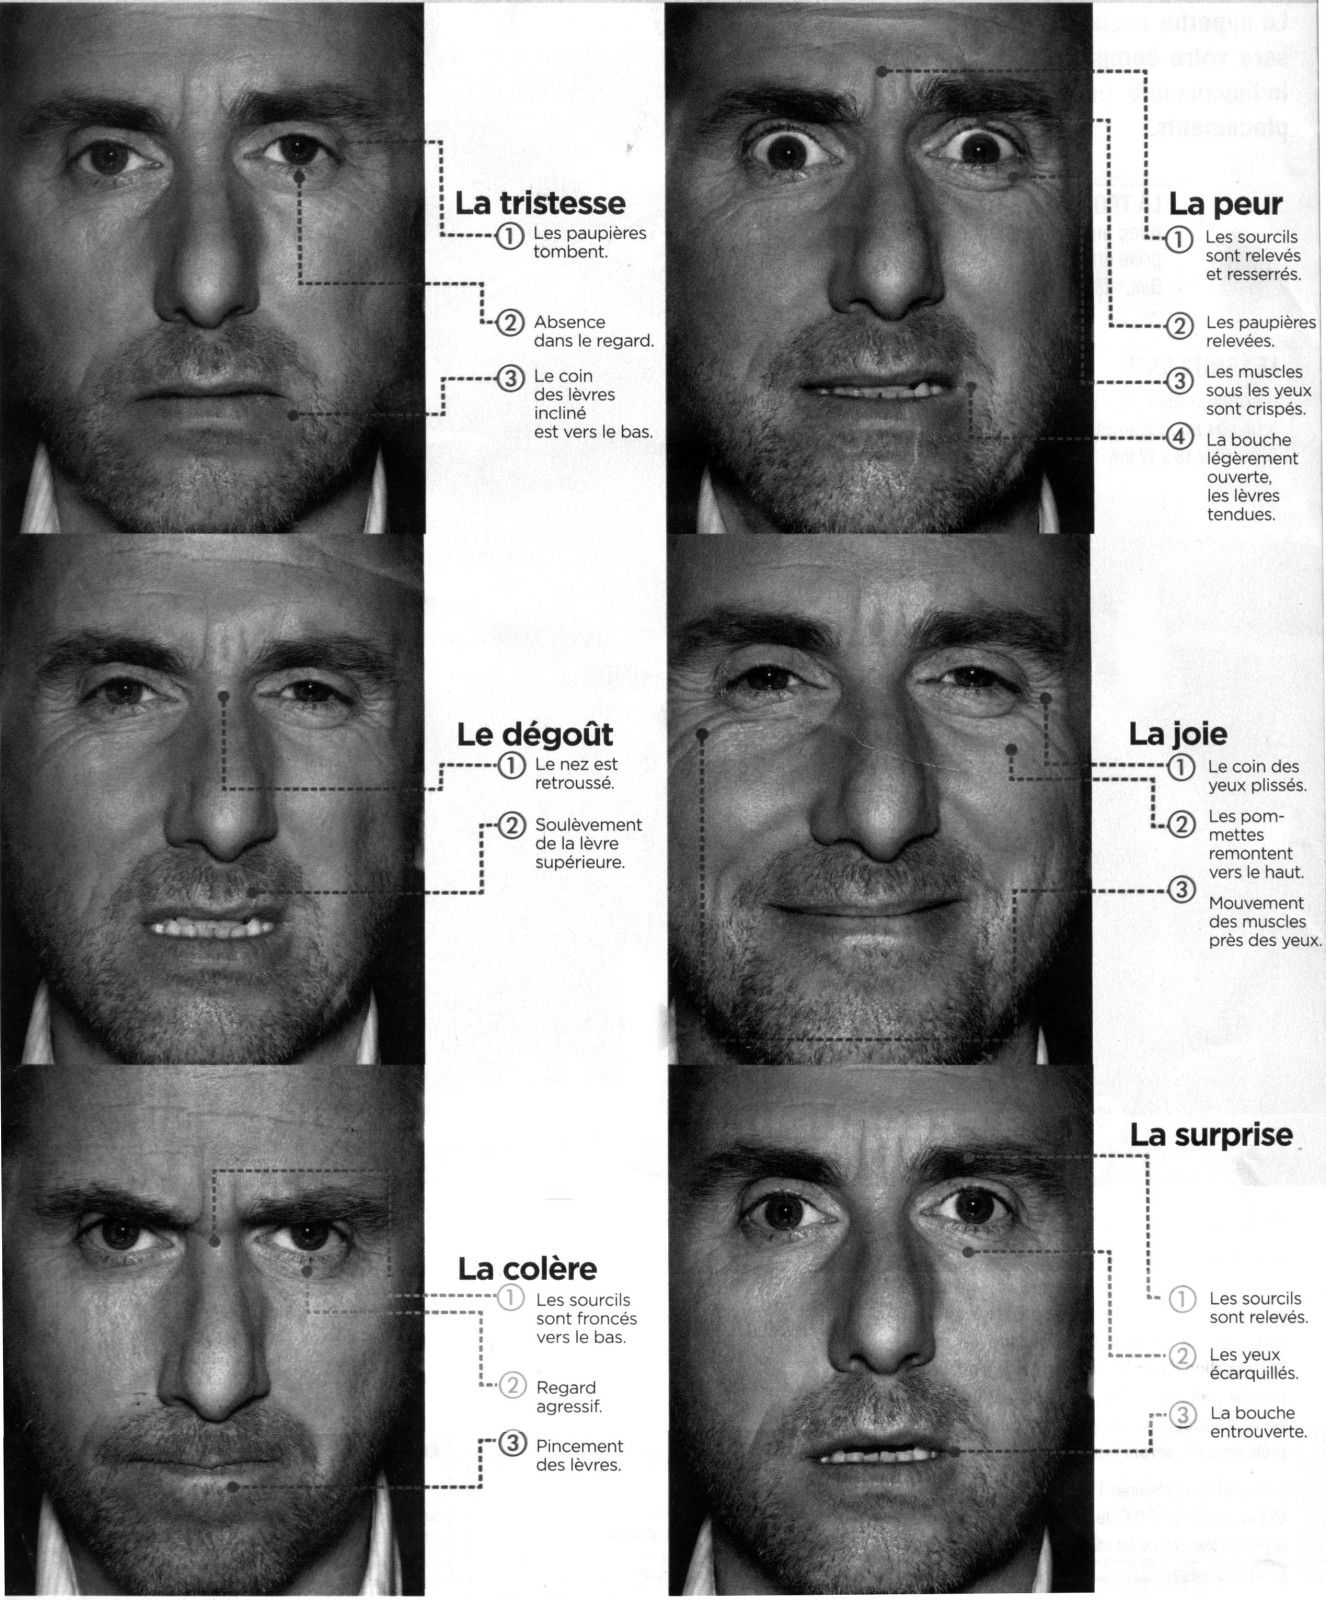
\includegraphics[width=14cm]{./Chapitre1/figures/ExpressionFacial.jpg}
  \caption{Marqueurs faciaux des 6 émotions primaires d'Ekman. In Lie To Me.}
  \label{fig:expressionFacial}
\end{figure}

Il est possible de capter beaucoup d'informations à partir du comportement et du corps de l'humain. %sur le visage et dans l'attitude d'une personne.
Nos expressions faciales notamment permettent de véhiculer les émotions primaires telles que la peur ou la colère comme montré dans la figure~\ref{fig:expressionFacial} en mettant en jeu le positionnement des sourcils, la forme de la bouche, le plissement du front...
Par exemple, la tristesse se caractérise par des paupières tombantes, un regard absent et une bouche légèrement inclinée vers le bas selon le \textit{Facial Action Coding System} de Paul Ekman~\cite{Ekman1978}.

Bien que ces marqueurs ont été affirmés comme étant universels par Paul Ekman~\cite{Ekman1978}, de nombreuses études ont mis en doute ce postulat~\cite{Leys2010,Gendron2014}. En effet, certains indicateurs étant communs entre plusieurs émotions, des interlocuteurs peuvent se tromper dans l'analyse de l'émotion de la personne. Par exemple, la bouche ouverte peut signifier la peur mais également la surprise. Les expressions faciales sont contrôlables. En effet, il est tout à fait possible de simuler une émotion ou dans une moindre mesure, d'en cacher une en fonction de l’entraînement d'un individu. C'est le cas notamment des acteurs professionnels qui sont capables de simuler un grand nombre d'émotions.

Les expressions faciales sont, aujourd'hui encore, l'une des modalités les plus observées pour définir et reconnaître des émotions. Elles peuvent également servir à détecter des états dépressifs ou des mensonges par exemple~\cite{Suslow2001,Owayjan2012}.

Les positionnements du corps, qu'on peut appeler \textit{l'attitude} d'une personne permet également de reconnaître ses émotions. En effet, les comportements adoptés par un individu, notamment la posture, peuvent refléter de l'état émotionnel interne d'une personne. Ce phénomène, préssenti par Darwin~\cite{Darwin1872}, est expliqué dans les travaux de Frijda (1987)~\cite{Frijda1987} qui indique que les émotions sont présentes pour aider l'homme à agir : l'homme est caractérisé par une tendance à l'action qui se traduit par des émotions. Ainsi lors de la colère, la position du buste sera en avant, tandis que pour la peur, elle sera plus retrait. Mais ces caractéristiques faciales et comportementales ne sont pas les seules permettant de reconnaitre l'état émotionnel d'un individu.

\subsection{Les marqueurs physiologiques de l'émotion}
Comme nous l'avons vu précédemment, l'expression de l'émotion est étroitement liée au cerveau et donc au système nerveux~\cite{Dantzer2002}. En étudiant ce dernier, nous pouvons retrouver des marqueurs émotionnels. La peur par exemple commence par un influx nerveux qui engendre une augmentation du rythme cardiaque, qui va augmenter l'afflux sanguin, la sudation, l'apport en oxygène par une respiration plus rapide~\cite{Steimer2002}.

De manière non-exhaustive, nous pouvons citer le rythme cardiaque~\cite{Wiens2000}, la sudation, la température de la peau (à l'origine des joues rouges), l'activité cérébrale, le suivi du regard, le rythme de la respiration comme des marqueurs physiologiques de l'émotion~\cite{Maaoui2010,Levenson2003}. Certains de ces marqueurs physiologiques peuvent être quantifiés par des outils de mesure. L'électrocardiogramme (EG) permet de suivre l'évolution du rythme cardiaque, l'électroencéphalogramme (EEG) permet de détecter les zones d'activité du cerveau. Des capteurs de sudation et des thermomètres peuvent permettre de suivre la production de sueurs au niveau des mains ou la température cutanée. Tous ces indicateurs peuvent caractériser la présence ou l'absence d'émotion chez un individu.

\section{Conclusion}
Dans ce chapitre, nous avons défini l'émotion et les différentes théories qui proposent de la définir, en proposant notamment un point de vue chronologique. Nous avons détaillé les différentes representations des émotions qui sont adaptées à du traitement automatique.
% Nous considérons les émotions que l'on nomme satisfaction et frustration selon une dimension continue que nous avons appelée la dimension de satisfaction. Cette dernière a pour extremum la satisfaction et la frustration, avec un état neutre en son milieu.

Nous avons également défini les différentes modalités où l'émotion s'exprime. En revenant sur la demande industrielle à l'origine de cette thèse, nous n'avons que la voix comme vecteur d'émotion, puisqu'il s'agit d'analyser des enregistrements audio de conversation issues de centres d'appels. Dans le chapitre 3
%~\ref{chapitre3}
, nous allons explorer plus en détail la mise en place de solutions de reconnaissance automatique de l'émotion depuis la modalité vocale.
